%% LaTeX2e class for student theses
%% sections/content.tex
%% 
%% Karlsruhe Institute of Technology
%% Institute for Program Structures and Data Organization
%% Chair for Software Design and Quality (SDQ)
%%
%% Dr.-Ing. Erik Burger
%% burger@kit.edu
%%
%% Version 1.3.5, 2020-06-26

\chapter{Introduction}
\label{ch:Introduction}


\begin{quote}{Sundar Pichai}
\textit{AI is one of the most important things humanity is working on. It is more profound than [...] electricity or fire \cite{AIQuotePichai}}
\end{quote}

\section{Motivation}

\subsection{Need for explainable artificial intelligence in general}

Artificial Intelligence (AI) has been revolutionizing technology since computers were invented \cite{TimeLineOfAI}. For most of that time the limitation had been processing power, limiting the complexity of artificial intelligence. Therefore, except for the rare exception, artificial intelligence which was being run could be understood by reading the underlying code that defined it.


Past decades have seen tremendous increase in processing power (see \autoref{fig:topComp}) which has shifted the limitations of AI from computational to cognitive processing power.

\begin{figure}[H]
\centering
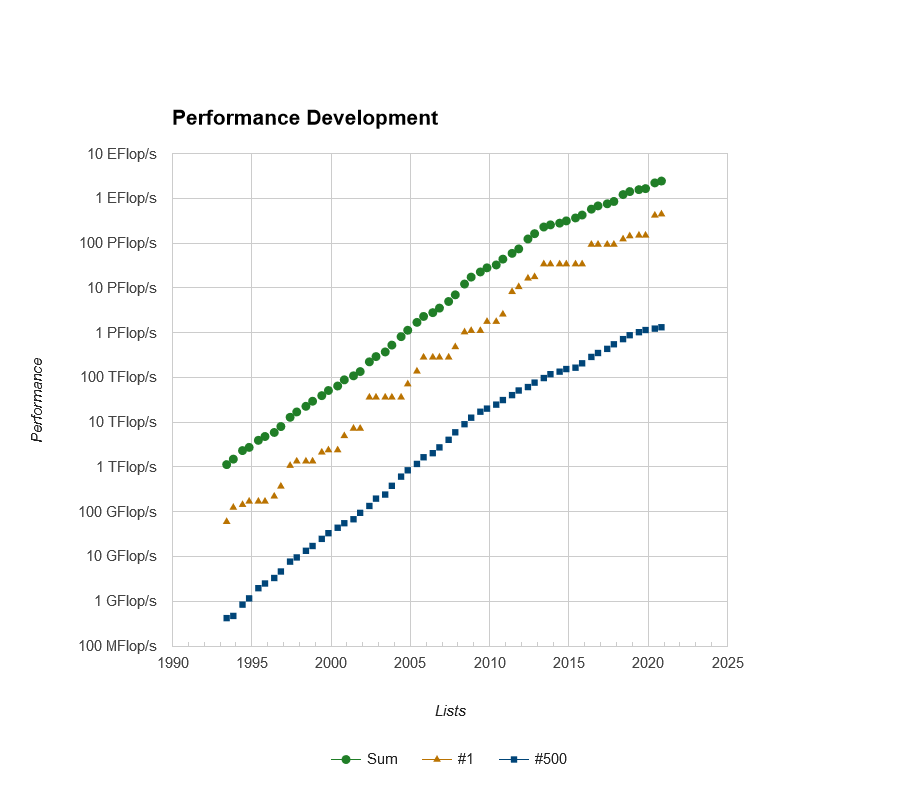
\includegraphics[width=\linewidth]{images/01_Intro/Top500.png}
\caption{Performance of the top 500 supercomputers over time \cite{top500}.}
\label{fig:topComp}
\end{figure}

This has culminated in the rise of a new type of algorithms, artificial neuronal networks. These apply a fundamentally different approach to AI. The human doesn't define the algorithm anymore but feeds data to a complex algorithm which writes its own program to solve a specific problem. These approaches have led to breakthroughs in many fields \cite{10.1145/3065386}. \par
While this step was arguably unavoidable for the advancement of AI, it poses its own challenges. Artificial neural networks can depend on millions of parameters \cite{szegedy2015going} which cannot, in their entirety, be understood due to our limited cognitive abilities. 

In \autoref{fig:complexity} I have tried to showcase the issue, modern day artificial neural networks are fundamentally more complex than any previous algorithms. 2013 is considered a breakthrough year in image recognition, with massive improvements in artificial neural network technology \cite{ILSVRC15}, but the exact moment the cognitive complexity barrier was breached is difficult to pinpoint.


\begin{figure}[H]
    \centering
    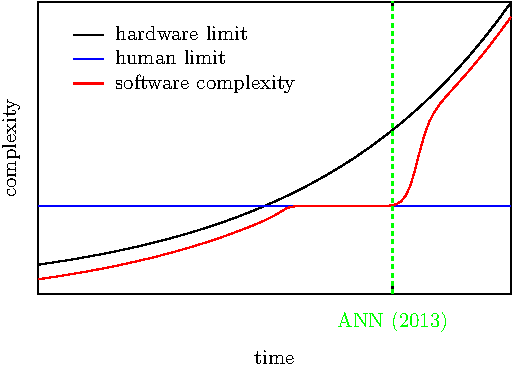
\includegraphics[width=0.8\linewidth]{images/01_Intro/Complexity.pdf}
    \caption{Breaking through the cognitive complexity barrier.}
    \label{fig:complexity}
\end{figure}

This inability to understand AI and algorithms in general poses a few fundamental problems.

\begin{itemize}
    \item How do we debug/improve algorithms we do not understand?
    \item How do we enforce laws on algorithms we do not understand?
    \item Can/should we use such an algorithm on applications where fatal errors are not permitted \textit{(ex: military applications)}
\end{itemize}



\subsection{Need for tools to analyse Explainable AI}

All of the above mentioned issues are being faced not only by scientists but more generally by software developers who do not have the luxury to spend months analysing one aspect of their software and require specialized tools to guide them. It can be argued that while neural networks where theorized decades ago, and could be implemented in hardware since the 2000s, it required frameworks and libraries like DistBelief, Tensorflow and more for their applications to become widespread and usable for most engineers and scientists. Theory and practicable tools need to go hand in hand to enable progress and in this context we wish to present our own framework to analyse explainable artificial intelligence tools.

\section{Applications for explainable AI}

The sceptical would argue that you cannot explain complex algorithms because they are by nature too complex to be understood in detail by a human. The argument would be, that if we were capable of explaining artificial neural networks, we could program them ourselves. While for certain cases this is true, it is not guaranteed. Multiple scenarios could happen:

\begin{enumerate}
    \item Developers just need a hint on how to solve a problem and an even incomplete explanation of a Neural Network enables them to code it in a humanly understandable way.
    \item We understand a fraction of how the artificial intelligence makes a decision but it is enough to disqualify it. This is especially important if some unwanted behaviour like biased \textit{(racist/sexist/...)} decisions are revealed.
    \item We understand a fraction of how the artificial intelligence makes a decision and the approach feels plausible to humans.
\end{enumerate}

Note that scenario three does not guarantee that no unwanted or even illegal behaviour is occurring. Similar to the quote from Edsger W. Dijkstra: \enquote{Program testing can be used to show the presence of bugs, but never to show their absence}, an incomplete explanation will never guarantee the absence of all issues opaque algorithms bring with them.
Nonetheless, XAI is fundamental if we wish to evaluate and compare algorithms with each other.


\section{Key questions}

In this bachelor thesis we will examine which approaches exist to understand artificial intelligence, meaning algorithms generated with the help of artificial neural networks, and we will explore one of these approaches in detail. In this context we will present a framework which has been developed by our team and myself to analyse XAI approaches and compare them with each other. Our key questions are which parameters are important for the usage of explainable artificial intelligence tools when applying them onto natural language in written form and how to tweak them to adjust unsatisfying explanations. Furthermore we will show how our framework can be used to create your own analysis.